\section{Results}
\label{sec:results}

\subsection{Depth encoding before learning}
\label{sec:res:encoders}

We first examine the untrained encoding mechanism, comparing the random phase plate with a defocused amplitude mask, a plate-free angular scan and an in-focus DMD. The phase plate produces approximately linear depth-dependent lateral shifts, with a shear pivot near its conjugate plane. Excitation sequences at fixed lateral positions decorrelate over approximately $1\um$ of axial separation. Detailed excitation and point-emitter diagnostics are given in the supplement.

With 32 illumination directions, maximum-likelihood localisation of point emitters with unknown brightness gives depth misassignment rates of 1.5--1.8\,\% for the phase plates, compared with 4.4--5.3\,\% for amplitude masks, 25\,\% for the tested DMD and 89\,\% without a plate. In neuronal reconstruction, the amplitude mask is competitive in centroid depth error, although the random phase plate achieves 0.4--1.2\,dB higher PSNR at $C=8$. These controls establish a useful untrained encoder. The following comparisons isolate the effect of learning by pairing the learned plate with its own random initialisation.

\subsection{Measurements distinguish axial arrangements}
\label{sec:res:measurements}

\begin{figure*}[t]
\centering
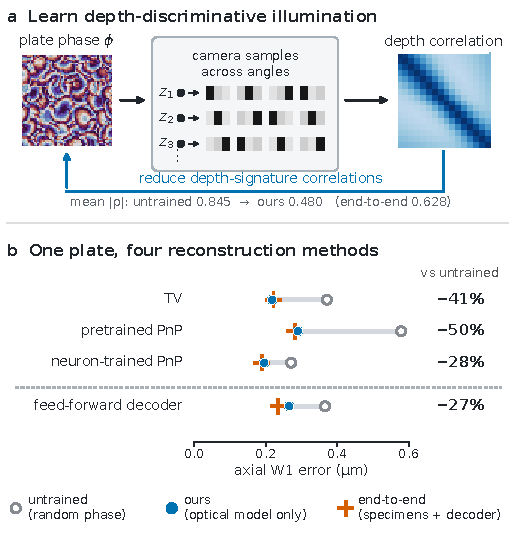
\includegraphics[width=0.43\linewidth,trim=0 96 0 11,clip]{overview.pdf}\hfill
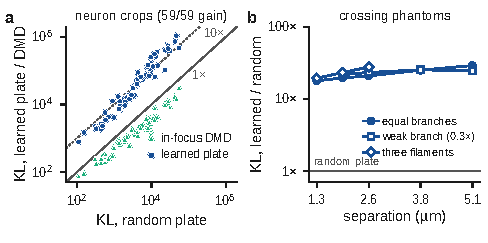
\includegraphics[width=0.55\linewidth]{measurement_separation.pdf}
\caption{\textbf{Learning changes the plate and increases measurement separation.} Left: phase maps and absolute depth-signature correlations before and after training. Right: brightness-profiled Poisson KL for (a) neuronal crops and (b) crossing phantoms, comparing each reference with a merged-depth alternative. Crop values average the five direction subsets. These tests use the expected measurements before reconstruction.}
\label{fig:measurement}
\end{figure*}

The phase maps and measurement signatures change during training (\cref{fig:measurement}). Mean absolute depth correlation falls between detector-integrated depth signatures from 0.84 to 0.48 at 32 illumination directions. To test a consequence beyond the training statistic, we compare each neuronal volume with an alternative that merges its layered columns while preserving their brightness and centroids (\cref{fig:measurement}). The learned plate increases brightness-profiled Poisson KL by a geometric mean factor of 10.0 (95\,\% CI: 8.7--11.8), with an increase in all 59 eligible crops. The corresponding factor is 10.4 with added background.

The gain is present before reconstruction. It measures stronger separation from these axial alternatives, without establishing unique recovery or showing that a merged volume agrees with the random plate's measurements. The phantom comparisons show the same trend, although large KL alone does not ensure recovery at every gap.

\subsection{Resolving crossing structures}
\label{sec:res:crossing}

The crossing-filament experiment tests whether improved measurements translate into recovery of distinct structures (\cref{fig:separation}). With TV and pretrained PnP, the smallest tested gap meeting the resolution and correct-ordering criterion falls from $3.84$ to $2.56\um$. The improvement holds at both axial centres, including the centre that does not coincide with the mirror pairing emphasised during training. Neither plate falsely splits the merged control in the tested cases.

Learned PnP retains a $3.84\um$ threshold, although learning increases success rates at smaller gaps. Learning also helps recover the weaker branch in unequal-intensity crossings, while closely spaced three-filament cases remain difficult. Thus, the learned plate improves controlled separation under two methods; it does not provide a common resolution threshold across all priors.

\subsection{Axial-profile recovery across reconstruction priors}
\label{sec:res:anyprior}

\begin{figure*}[t]
\centering
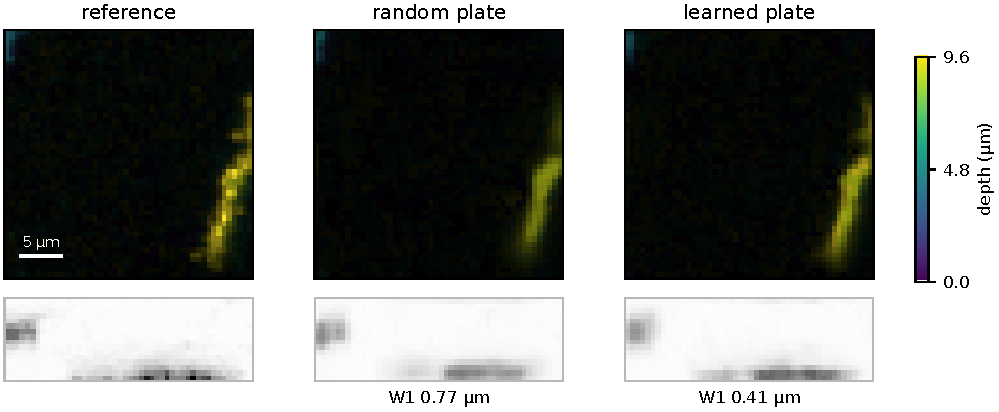
\includegraphics[width=0.92\linewidth]{neuron_profiles.pdf}
\caption{\textbf{Neuronal reconstruction with pretrained PnP.} Top: lateral maximum-intensity projections, coloured by the depth of the brightest voxel. Bottom: axial maximum-intensity projections. Each view uses a common display scale across the reference and reconstructions. The crop is selected by median W1 improvement across the three methods; draw 0 is shown at $C=8$ and equal dose. Selection and all-decoder views are given in the supplement.}
\label{fig:anyprior}
\end{figure*}

\begin{table}[t]
\centering\small
\setlength{\tabcolsep}{3pt}
\resizebox{\linewidth}{!}{\begin{tabular}{@{}l cc c@{}}\toprule
& \multicolumn{2}{c}{axial W1 ($\mu$m) $\downarrow$} & reduction [95\,\% CI]\\
\cmidrule(lr){2-3}
decoder & random & learned & learned vs random\\\midrule
TV & 0.371 & 0.218 & $41$\,\% [$38$, $45$]\\
pretrained PnP & 0.579 & 0.290 & $50$\,\% [$47$, $53$]\\
learned PnP & 0.271 & 0.195 & $28$\,\% [$26$, $29$]\\
\bottomrule\end{tabular}
}
\caption{\textbf{Axial-profile recovery at eightfold measurement compression.} Mean over 60 crops from six cells, with five direction subsets per crop and equal deposited excitation dose. Relative reductions compare paired means; intervals resample cells. All three methods improve on every crop.}
\label{tab:anyprior}
\end{table}

The learned plate improves mean axial W1 under TV, pretrained PnP and learned PnP by 41\,\%, 50\,\% and 28\,\%, respectively (\cref{fig:anyprior,tab:anyprior}). All cell-bootstrap intervals exclude zero, and all 60 crops improve under each method. The evaluation includes 48 randomly selected crops added after decoder parameters were fixed, alongside the 12 prespecified crops. A second optical optimisation seed gives comparable W1 reductions of 41\,\%, 50\,\% and 29\,\% from the same initial plate.

Centroid error also falls by 30--54\,\%, and PSNR increases by 1.6--1.8\,dB. Both the axial distributions and their centroids are recovered more accurately. On layered columns, the strictly reproduced TV comparison gives a 34\,\% W1 reduction; detailed subset results and re-evaluation checks are provided in the supplement.

The in-focus DMD remains a useful control for weak axial encoding. On the 12 prespecified crops, its W1 is $2.24$--$2.38\um$ across the three decoders, close to the uniform-depth reference of $2.27\um$. These results concern the tested in-focus encoder, rather than DMD-based imaging systems in general.

\subsection{Measurement and dose trade-offs}
\label{sec:res:efficiency}

\begin{figure}[t]
\centering
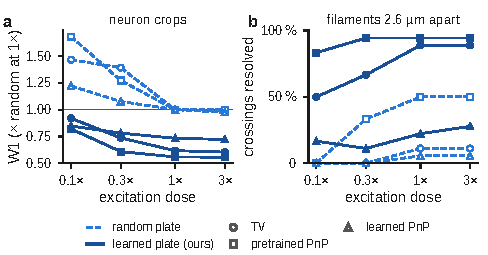
\includegraphics[width=\linewidth]{dose.pdf}
\caption{\textbf{Benefits at reduced excitation dose.} (a) Neuronal W1 relative to each decoder's random-plate result at full dose, evaluated on the 12 prespecified crops. (b) Success rates for crossing filaments $2.56\um$ apart. Solid: learned plate; dashed: random plate. Exposure varies at a fixed count of 32 illumination directions.}
\label{fig:dose}
\end{figure}

On the 12 prespecified crops, the learned plate lowers W1 at all tested compression factors ($C=1,4,8$). At equal total deposited dose, its 32-direction measurements outperform the random plate's 256-direction measurements under TV ($0.196$ versus $0.249\um$) and pretrained PnP ($0.277$ versus $0.413\um$). Learned PnP gives similar means ($0.206$ versus $0.203\um$), without evidence establishing equivalence. Here, fewer images receive longer exposures, so the measurement reduction does not imply an equal reduction in acquisition time.

At a fixed 32 directions, the learned plate at 0.3 times the excitation dose achieves lower W1 than the random plate at full dose (\cref{fig:dose}). Reductions are 26\,\% [20, 33] with TV, 39\,\% [34, 45] with pretrained PnP and 22\,\% [16, 28] with learned PnP. These are paired comparisons at the tested dose levels. The small changes between full and triple dose describe the selected reconstruction protocols, rather than a fundamental photon limit.

\subsection{Optical objectives and robustness}
\label{sec:res:objective}

\begin{table}[t]
\centering\small
\setlength{\tabcolsep}{3pt}
\resizebox{\linewidth}{!}{\begin{tabular}{@{}l cc c@{}}\toprule
& \multicolumn{2}{c}{axial W1 ($\mu$m) $\downarrow$} & ours vs this\\
\cmidrule(lr){2-3}
objective & $C=1$ & $C=8$ & reduction [95\,\% CI]\\\midrule
random plate & 0.203 & 0.282 & $27$\,\% [$20$, $34$]\\
worst-case coherence & 0.172 & 0.238 & $13$\,\% [$12$, $15$]\\
depth Fisher information & 0.164 & 0.240 & $14$\,\% [$12$, $17$]\\
decorrelation, uncentred & 0.142 & 0.207 & $0$\,\% [$-1$, $1$]\\
depth decorrelation (ours) & 0.142 & 0.206 & --\\
\bottomrule\end{tabular}
}
\caption{\textbf{Controlled comparison of optical training objectives.} Learned-PnP W1 on the 12 prespecified crops. Plates share the initial phase, sampling and optimisation budget, with validation tuning for each encoder. The final column compares our plate with each row at $C=8$.}
\label{tab:objectives}
\end{table}

We compare depth decorrelation with worst-case coherence, depth Fisher information and an uncentred variant (\cref{tab:objectives}). All objectives improve upon the random plate. Across both optimisation seeds and all three decoders, our objective gives 13--20\,\% lower W1 at $C=8$ than the tested coherence and Fisher-information implementations. Centring has negligible effect. These comparisons favour depth decorrelation under the tested training conditions.

\paragraph{Noise.} With background and read noise, W1 reductions remain 30\,\%, 53\,\% and 27\,\% for TV, pretrained PnP and learned PnP. Gains also persist when both encoders receive one tenth of the reference dose. The full noise model and paired results are given in the supplement.

\paragraph{Alignment and calibration.}
\label{sec:res:tolerance}
For learned PnP, plate-distance offsets of $\pm0.5\um$ retain W1 reductions of 27--28\,\% after updating the forward model. Uncalibrated pointing errors of 0.005--0.01 in direction cosine retain reductions of 13--20\,\%. In contrast, uncalibrated plate-distance or lateral-position errors eliminate the learned advantage; a one-feature lateral shift makes W1 11\,\% worse than the random plate (95\,\% CI: 2--23\,\%). Accurate optical registration is therefore necessary to preserve the benefit.
